\chapter{Chapter}\label{chap:chapter1}
\section{Section}\label{sec:sec1}
	\subsection{Subsection}\label{sub:sub1}
		\begin{table}[!h]
			\renewcommand{\arraystretch}{1.2}
			\centering
			\caption{Template Table}
			\begin{zebratabular}{m{6cm} m{5.8cm} m{3.2cm}}
				\rowcolor{gray}
				\textbf{Column 1}	& \textbf{Column 2}										& \textbf{Column 3} \\
				Something			& interesting using citations \cite{micropumpsMGD2000}	& great! \\ 
				Something			& interesting using an acronym \ac{TMPL}				& very nice! \\ 
			\end{zebratabular}
			\renewcommand{\arraystretch}{1.0}
			\label{tab:template}
		\end{table}

		\subsubsection{Subsubsection}\label{subsub:subsub1}
			\begin{figure}[H]
				\centering
				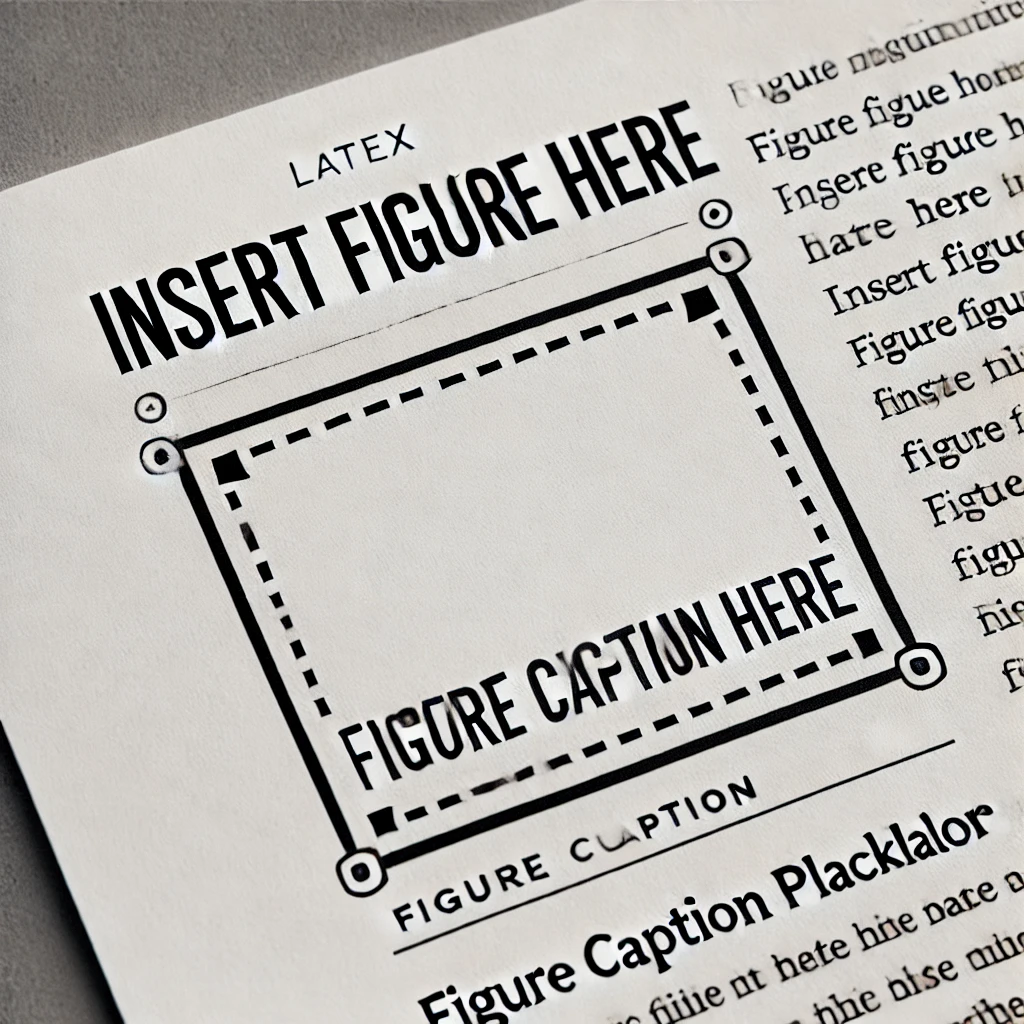
\includegraphics[width=.7\textwidth]{./figure/template_figure.png}
				\caption{Template Figure}
				\label{fig:template}
			\end{figure}
		\paragraph{Paragraph}
	
			\tikz \datavisualization 	data group {template} = {
				data [set=templatecol1, headline={x, y, z}, read from file=./figure/plots/dummy_data.csv]
				data [set=templatecol2, headline={x, z, y}, read from file=./figure/plots/dummy_data.csv]
			};

			\begin{figure}[h]
				\centering
				\begin{tikzpicture}
					\datavisualization [scientific axes,
										x axis={length=.8\textwidth, grid, label={Time [s]}},
										y axis={min value=-0.5, max value=2.5, length= 4cm, grid, label={Amplitude [V]}},
										visualize as line/.list={templatecol1,templatecol2},
										templatecol1= {label in legend={text=Input}},
										templatecol2= {label in legend={text=Output}},
										style sheet=strong colors]
				data group {template};

				\end{tikzpicture}
				\caption{Template Plot}
				\label{plt:template}
			\end{figure}
